\documentclass[a4paper, 11pt]{article}
\usepackage[UTF8, scheme = plain]{ctex}
\usepackage{amsmath}
\usepackage{graphicx}
\usepackage{geometry}
\usepackage{listings}
\usepackage{xcolor}
\usepackage{bm}
\usepackage{caption,subcaption}
\geometry{scale=0.8}
\linespread{1.5}
\usepackage[colorlinks,linkcolor=red,anchorcolor=blue]{hyperref}
\usepackage{listings}
\usepackage{enumitem}
\usepackage{algorithm}
\usepackage{algorithmicx}
\usepackage{algpseudocode}

\usepackage{amssymb}

\lstset{
language={Python},
frame=shadowbox,
breaklines=true,
 numbers=left,
 backgroundcolor=\color[RGB]{245,245,244},
 rulesepcolor=\color{red!20!green!20!blue!20},
 numberstyle={\color[RGB]{0,192,192}\tiny},
 basicstyle=\footnotesize
 }
\setenumerate[1]{itemsep=0pt,partopsep=0pt,parsep=\parskip,topsep=0pt}
\setitemize[1]{itemsep=0pt,partopsep=0pt,parsep=\parskip,topsep=0pt}
\setdescription{itemsep=0pt,partopsep=0pt,parsep=\parskip,topsep=0pt}


\title{	
\normalfont \normalsize
\textsc{School of Data and Computer Science, Sun Yat-sen University} \\ [25pt] %textsc small capital letters
\rule{\textwidth}{0.5pt} \\[0.4cm] % Thin top horizontal rule
\huge  E18 Deep Q-Learning (C++/Python)\\ % The assignment title
\rule{\textwidth}{2pt} \\[0.5cm] % Thick bottom horizontal rule
\author{Suixin Ou \and Yangkai Lin}
\date{\normalsize\today}
}

\begin{document}
\maketitle
\tableofcontents
\newpage

\section{Deep Q-Network (DQN) }
We consider tasks in which an agent interacts with an environment $\mathcal{E}$, in this case the Atari emulator, in a sequence of actions, observations and rewards. 
At each time-step the agent selects an action $a_t$ from the set of legal game actions, $\mathcal{A}=\{1, ..., K \}$. The action is passed to the emulator and modifies its internal state and the game score. In general $\mathcal{E}$ may be stochastic. The emulator's internal state is not observed by the agent,  instead it observes an image $x_t\in\mathbb{R}^d$ from the emulator, which is a vector of raw pixel values representing the current screen. In addition it receives a reward $r_t$ representing the change in game score. Note that in general the game score may depend on the whole prior sequence of actions and observations; feedback about an action may only be received after many thousands of time-steps have elapsed. 

Since the agent only observes images of the current screen, the task is partially observed and many emulator states are perceptually aliased, i.e. it is impossible to fully understand the current situation from only the current screen $x_t$. We therefore consider sequences of actions and observations, $s_t = {x_1, a_1, x_2, ..., a_{t-1}, x_t}$, and learn game strategies that depend upon these sequences. All sequences in the emulator are assumed to terminate in a finite number of time-steps. This formalism gives rise to a large but finite Markov decision process (MDP) in which each sequence is a distinct state. As a result, we can apply standard reinforcement learning methods for MDPs, simply by using the complete sequence $s_t$ as the state representation at time $t$.

The goal of the agent is to interact with the emulator by selecting actions in a way that maximises future rewards. We make the standard assumption that future rewards are discounted by a factor of $\gamma$ per time-step, and define the future discounted \emph{return} at time $t$ as $R_t = \sum_{t'=t}^{T} \gamma^{t'-t} r_{t'}$, where $T$
is the time-step at which the game terminates. We define the optimal action-value function $Q^*(s,a)$ as the maximum expected return achievable by following any strategy, after seeing some sequence $s$ and then taking some action $a$, $Q^*(s,a) = \max_{\pi} \mathbb E[R_t | s_t=s, a_t=a, \pi ]$, where $\pi$ is a policy mapping sequences to actions (or distributions over actions).

The optimal action-value function obeys an important identity known as the \emph{Bellman equation}. This is based on the following intuition: if the optimal value $Q^*(s',a')$ of the sequence $s'$ at the next time-step was known for all possible actions $a'$, then the optimal strategy is to select the action $a'$ maximising the expected value of $r + \gamma Q^*(s',a')$,
%
\begin{align}
Q^*(s,a) &= \mathbb E_{s' \sim \mathcal{E}}[r + \gamma \max_{a'} Q^*(s', a') \Big| s, a]
\end{align}
%
The basic idea behind many reinforcement learning algorithms is to estimate the action-value function, by using the Bellman equation as an iterative update, $Q_{i+1}(s,a) = \mathbb{E}\left[ r + \gamma \max_{a'} Q_i(s', a') | s, a \right]$. Such \emph{value iteration} algorithms converge to the optimal action-value function, $Q_i \rightarrow Q^*$ as $i \rightarrow \infty$. In practice, this basic approach is totally impractical, because the action-value function is estimated separately for each sequence, without any generalisation. Instead, it is common to use a function approximator to estimate the action-value function, $Q(s,a; \theta) \approx Q^*(s,a)$. In the reinforcement learning community this is typically a linear function approximator, but sometimes a non-linear function approximator is used instead, such as a neural network. We refer to a neural network function approximator with weights $\theta$ as a Q-network. A Q-network can be trained by minimising a sequence of loss functions $L_i(\theta_i)$ that changes at each iteration $i$,
%
\begin{align}
L_i\left(\theta_i\right) &= \mathbb E_{s,a \sim \rho(\cdot)}[\left(y_i - Q \left(s,a ; \theta_i \right) \right)^2],
\label{eq:q-learning-loss}
\end{align}
%
where $y_i = \mathbb E_{s' \sim \mathcal{E}}[r + \gamma \max_{a'} Q(s', a'; \theta_{i-1}) | s, a ]$ is the target for iteration $i$ and $\rho(s,a)$ is a probability distribution over sequences $s$ and actions $a$ that we refer to as the \emph{behaviour distribution}. The parameters from the previous iteration $\theta_{i-1}$ are held fixed when optimising the loss function $L_i\left(\theta_i\right)$. 
Note that the targets depend on the network weights; this is in contrast with the targets used for supervised learning, which are fixed before learning begins.
% This can lead to feedback effects and even divergence during training, which is a major reason why reinforcement learning is more challenging than supervised learning.
Differentiating the loss function with respect to the weights we arrive at the following gradient,
%
\begin{align}
\nabla_{\theta_i} L_i\left(\theta_i\right) &= \mathbb{E}_{s,a \sim \rho(\cdot); s' \sim \mathcal{E}} \left[ \left( r + \gamma \max_{a'} Q(s', a'; \theta_{i-1}) - Q(s,a ; \theta_i ) \right) \nabla_{\theta_i} Q(s,a;\theta_{i}) \right] .
\label{eq:q-learning-gradient}
\end{align}
%
Rather than computing the full expectations in the above gradient, it is often computationally expedient to optimise the loss function by stochastic gradient descent. If the weights are updated after every time-step, and the expectations are replaced by single samples from the behaviour distribution $\rho$ and the emulator $\mathcal{E}$ respectively, then we arrive at the familiar \emph{Q-learning} algorithm. 

Note that this algorithm is \emph{model-free}: it solves the reinforcement learning task directly using samples from the emulator $\mathcal{E}$, without explicitly constructing an estimate of $\mathcal{E}$. It is also \emph{off-policy}: it learns about the greedy strategy $a = \max_{a} Q(s,a;\theta)$, while following a behaviour distribution that ensures adequate exploration of the state space. In practice, the behaviour distribution is often selected by an $\epsilon$-greedy strategy that follows the greedy strategy with probability $1 - \epsilon$ and selects a random action with probability $\epsilon$.

\begin{algorithm}[ht]
\begin{algorithmic}
\State Initialize replay memory $\mathcal{D}$ to capacity $N$
\State Initialize action-value function $Q$ with random weights
%\State Require preprocessor $h(s)$ that maps histories to fixed-length representations.
\For{episode $=1,M$} 
\State Initialise sequence $s_1 = \{x_1\}$ and preprocessed sequenced $\phi_1 = \phi(s_1)$
\For {$t=1,T$}
	\State With probability $\epsilon$ select a random action $a_t$
	\State otherwise select $a_t = \max_{a} Q^*(\phi(s_t), a; \theta)$
	\State Execute action $a_t$ in emulator and observe reward $r_t$ and image $x_{t+1}$
	\State Set $s_{t+1} = s_t,a_t,x_{t+1}$ and preprocess $\phi_{t+1} = \phi(s_{t+1})$
	\State Store transition $\left(\phi_t,a_t,r_t,\phi_{t+1}\right)$ in $\mathcal{D}$
	%\For {$k=1$ to $K$}
	\State Sample random minibatch of transitions $\left(\phi_j,a_j,r_j,\phi_{j+1}\right)$ from $\mathcal{D}$
	\State Set
	$y_j =
    \left\{
    \begin{array}{l l}
      r_j  \quad & \text{for terminal } \phi_{j+1}\\
      r_j + \gamma \max_{a'} Q(\phi_{j+1}, a'; \theta) \quad & \text{for non-terminal } \phi_{j+1}
    \end{array} \right.$
	\State Perform a gradient descent step on $\left(y_j - Q(\phi_j, a_j; \theta) \right)^2$ 
	according to equation~\ref{eq:q-learning-gradient}
	%\EndFor
\EndFor
\EndFor
\end{algorithmic}
\caption{Deep Q-learning with Experience Replay}
\label{alg}
\end{algorithm}
\newpage
\section{Deep Learning Flappy Bird }
\subsection*{Overview}
This project (\url{https://github.com/yenchenlin/DeepLearningFlappyBird}) follows the description of the Deep Q Learning algorithm described in \emph{Playing Atari with Deep Reinforcement Learning} and shows that this learning algorithm can be further generalized to the notorious Flappy Bird.

\subsection*{Installation Dependencies:}

\begin{itemize}
\itemsep1pt\parskip0pt\parsep0pt
\item
  Python 2.7 or 3
\item
  TensorFlow 0.7
\item
  pygame
\item
  OpenCV-Python
\end{itemize}

\href{https://github.com/yenchenlin/DeepLearningFlappyBird\#how-to-run}{}

\subsection*{How to Run?}

\begin{verbatim}
git clone https://github.com/yenchenlin1994/DeepLearningFlappyBird.git
cd DeepLearningFlappyBird
python deep_q_network.py
\end{verbatim}

\href{https://github.com/yenchenlin/DeepLearningFlappyBird\#what-is-deep-q-network}{}

\subsection*{What is Deep Q-Network?}

It is a convolutional neural network, trained with a variant of
Q-learning, whose input is raw pixels and whose output is a value
function estimating future rewards.

For those who are interested in deep reinforcement learning, I highly
recommend to read the following post: \href{http://www.nervanasys.com/demystifying-deep-reinforcement-learning/}{Demystifying Deep Reinforcement Learning}

\href{https://github.com/yenchenlin/DeepLearningFlappyBird\#deep-q-network-algorithm}{}

\subsection*{Deep Q-Network Algorithm}

The pseudo-code for the Deep Q Learning algorithm 
can be found below:

\begin{verbatim}
Initialize replay memory D to size N
Initialize action-value function Q with random weights
for episode = 1, M do
    Initialize state s_1
    for t = 1, T do
        With probability ϵ select random action a_t
        otherwise select a_t=max_a  Q(s_t,a; θ_i)
        Execute action a_t in emulator and observe r_t and s_(t+1)
        Store transition (s_t,a_t,r_t,s_(t+1)) in D
        Sample a minibatch of transitions (s_j,a_j,r_j,s_(j+1)) from D
        Set y_j:=
            r_j for terminal s_(j+1)
            r_j+γ*max_(a^' )  Q(s_(j+1),a'; θ_i) for non-terminal s_(j+1)
        Perform a gradient step on (y_j-Q(s_j,a_j; θ_i))^2 with respect to θ
    end for
end for
\end{verbatim}

\href{https://github.com/yenchenlin/DeepLearningFlappyBird\#experiments}{}

\subsection*{Experiments}

\textbf{Environment}

Since deep Q-network is trained on the raw pixel values observed from the game screen at each time step, so removing the background appeared in the original game can make it converge faster.

This process can be visualized as the following figure:
\begin{figure}
\centering
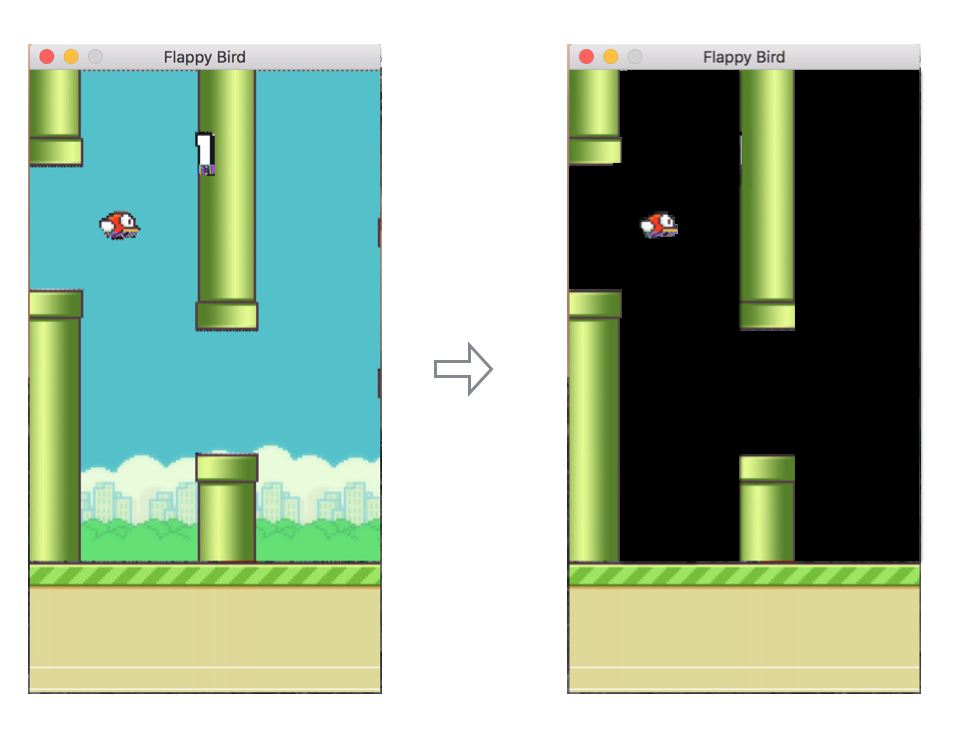
\includegraphics[width=0.9\textwidth]{Pic/preprocess}
\end{figure}

\textbf{Network Architecture}

I first preprocessed the game screens with following steps:

\begin{enumerate}
\itemsep1pt\parskip0pt\parsep0pt
\item
  Convert image to grayscale
\item
  Resize image to 80x80
\item
  Stack last 4 frames to produce an $80\times 80\times 4$ input array for network
\end{enumerate}

The architecture of the network is shown in the figure below. The first
layer convolves the input image with an $8\times 8\times 4\times 32$ kernel at a stride size
of 4. The output is then put through a $2\times 2$ max pooling layer. The second
layer convolves with a $4\times 4\times 32\times 64$ kernel at a stride of 2. We then max
pool again. The third layer convolves with a $3\times 3\times 64\times 64$ kernel at a
stride of 1. We then max pool one more time. The last hidden layer consists of 256 fully connected ReLU nodes.
\begin{figure}[ht]
\centering
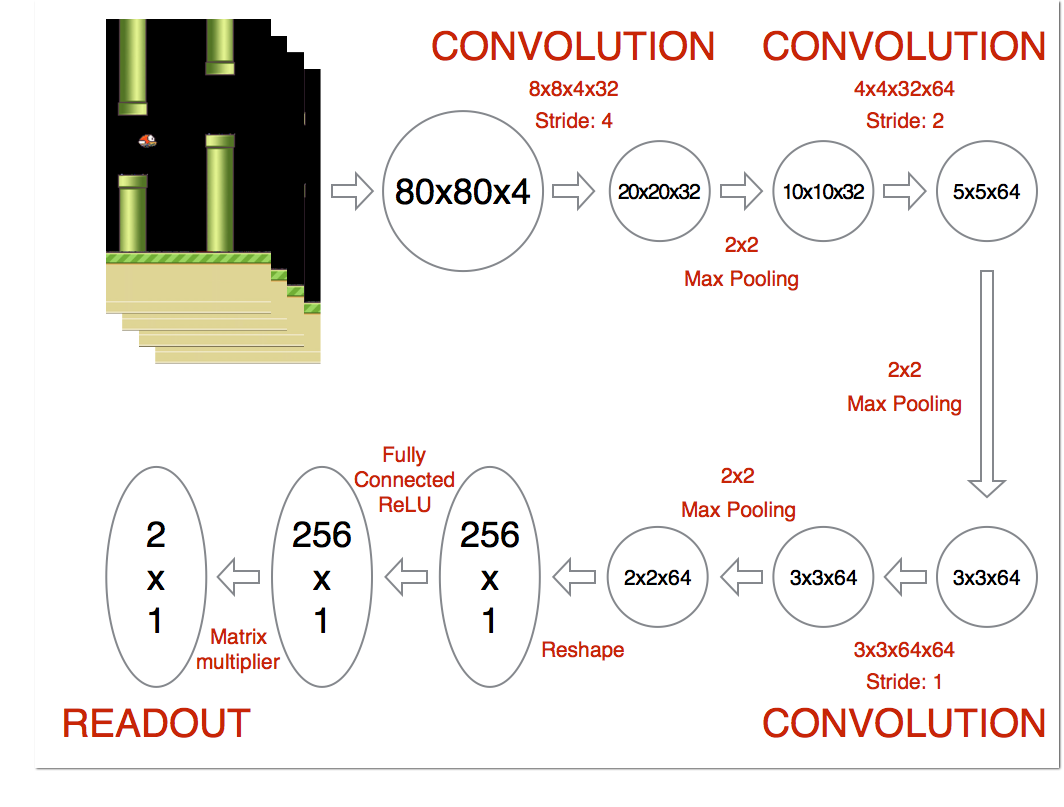
\includegraphics[width=16cm]{Pic/network}
\end{figure}

The final output layer has the same dimensionality as the number of valid actions which can be performed in the game, where the 0th index always corresponds to doing nothing. The values at this output layer
represent the $Q$ function given the input state for each valid action. At each time step, the network performs whichever action corresponds to the highest $Q$ value using a $\epsilon$ greedy policy.

\textbf{Training}

At first, I initialize all weight matrices randomly using a normal distribution with a standard deviation of 0.01, then set the replay memory with a max size of 500,00 experiences.

I start training by choosing actions uniformly at random for the first 10,000 time steps, without updating the network weights. This allows the
system to populate the replay memory before training begins.

I linearly anneal $\epsilon$from 0.1 to 0.0001 over the course of the next 3000,000 frames. The reason why I set it this way is that agent can choose an action every 0.03s (FPS=30) in our game, high $\epsilon$ will make it \textbf{flap} too much and thus keeps itself at the top of the game screen and finally bump the pipe in a clumsy way. This condition will make Q function converge relatively slow since it only start to look other conditions when $\epsilon$ is low. However, in other games, initialize $\epsilon$ to 1 is more reasonable.

During training time, at each time step, the network samples minibatches of size 32 from the replay memory to train on, and performs a gradient step on the loss function described above using the Adam optimization
algorithm with a learning rate of 0.000001. After annealing finishes, the network continues to train indefinitely, with $\epsilon$ fixed at 0.001.

\section{Tasks}
\begin{enumerate}
	\item Please implement a DQN to play the Flappy Bird game.
	\item You can refer to the codes in \url{https://github.com/yenchenlin/DeepLearningFlappyBird}
	\item Please submit a file named \texttt{E18\_YourNumber.zip}, which should includes the code files and the result pictures, and send it to \texttt{ai\_2020@foxmail.com}
\end{enumerate}
\section{Codes and Results}
\subsection{Codes}
最开始报这个错:
\begin{lstlisting}
AttributeError: module 'tensorflow' has no attribute 'InteractiveSession'
\end{lstlisting}
经上网查询,得知其因为tensorflow版本不同导致,需将:
\begin{lstlisting}
import tensorflow as tf
\end{lstlisting}
改为:
\begin{lstlisting}
import tensorflow.compat.v1 as tf
tf.disable_v2_behavior()
\end{lstlisting}
它和普通的Q-learning的区别在于,Q-learning用一个Q表来记录某状态下做某动作的得分,在状态空间很大动作很多的情况下这是很耗内存的。而Deep Q-learning则利用一个神经网络来估计Q表,每一步用梯度下降来更新神经网络:
\begin{lstlisting}
# perform gradient step
train_step.run(feed_dict = {
    y : y_batch,
    a : a_batch,
    s : s_j_batch}
)
\end{lstlisting}
\subsection{Results}
该代码有提前训练好的结果,在此展示:\href{run:run.mp4}{run.mp4}。

\end{document} 
%%% Local Variables:
%%% mode: latex
%%% TeX-master: t
%%% End:
